Este anexo recoge las figuras que, a modo complementario, se utilizan para la justificación de la elección de la 
agregación de los datos de días laborables.


\begin{figure}[H]
 \centering
    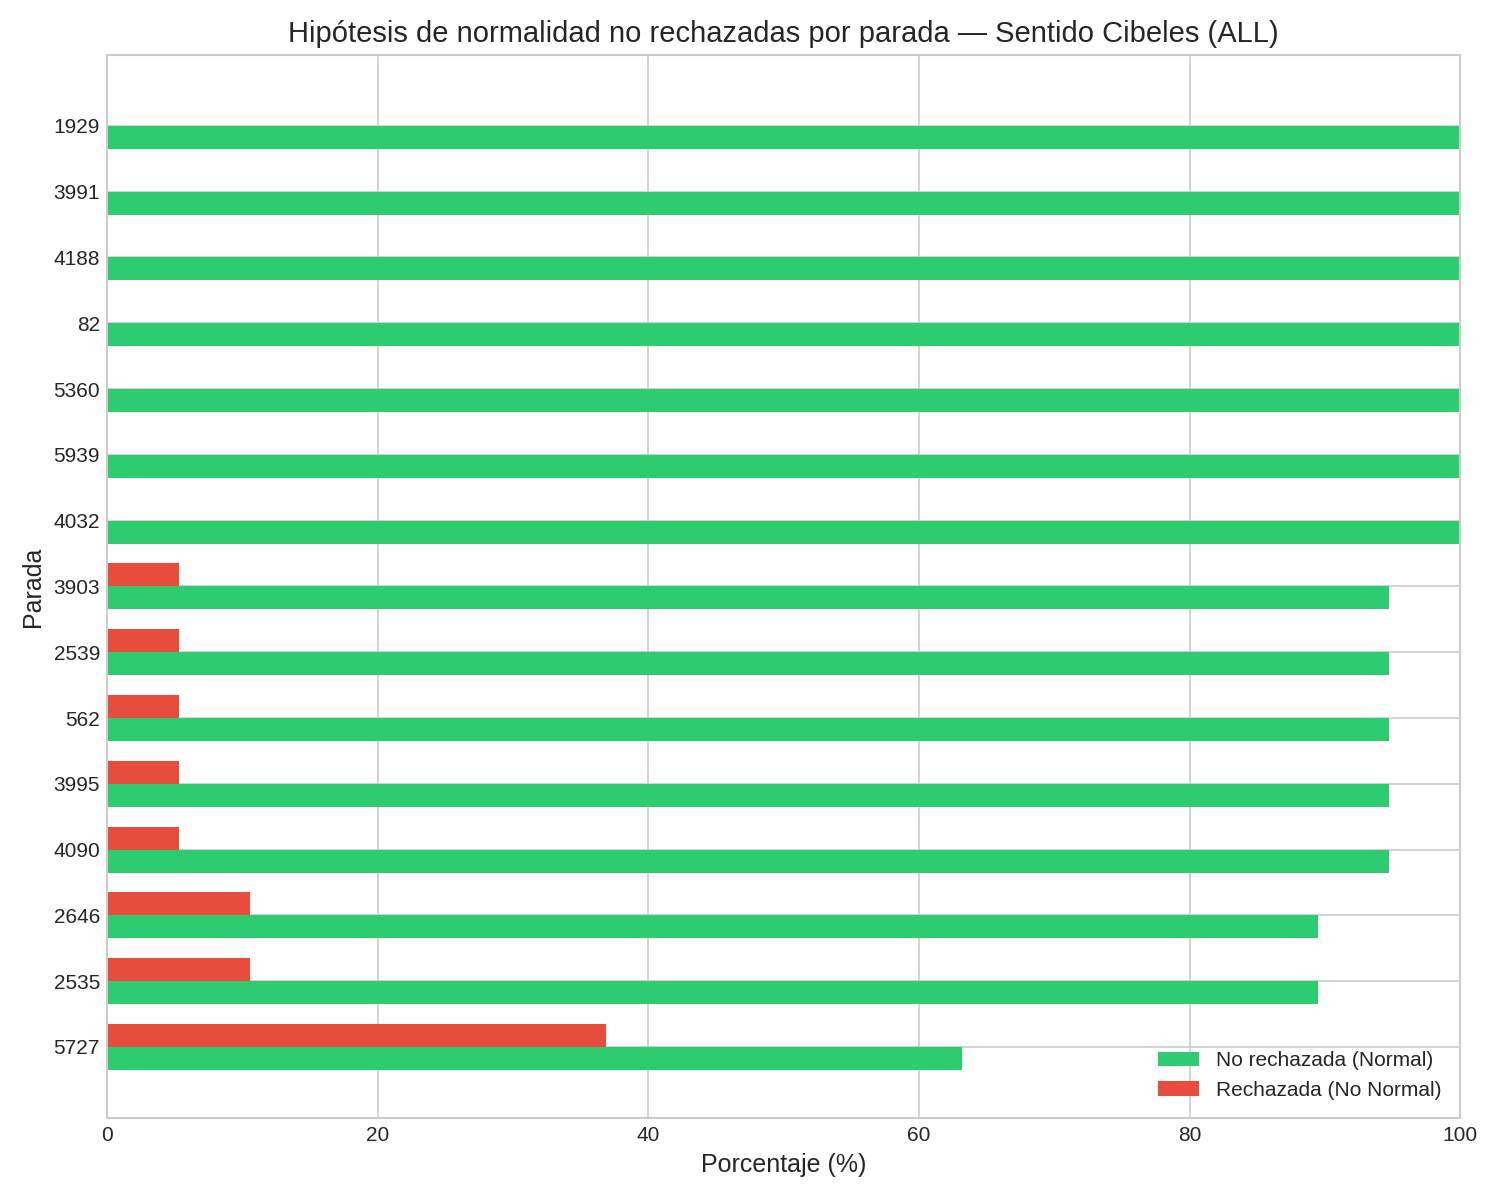
\includegraphics[width=\textwidth]{imagenes/to_A/normality_stop_ALL.png}
\caption{Porcentaje de no rechazo de hipótesis de normalidad por parada en sentido Cibeles con datos agregados.}
\par\vspace{4pt}{\footnotesize Fuente: elaboración propia.}\label{fig:normality_toA_all}
\end{figure}

\begin{figure}[H]
 \centering
    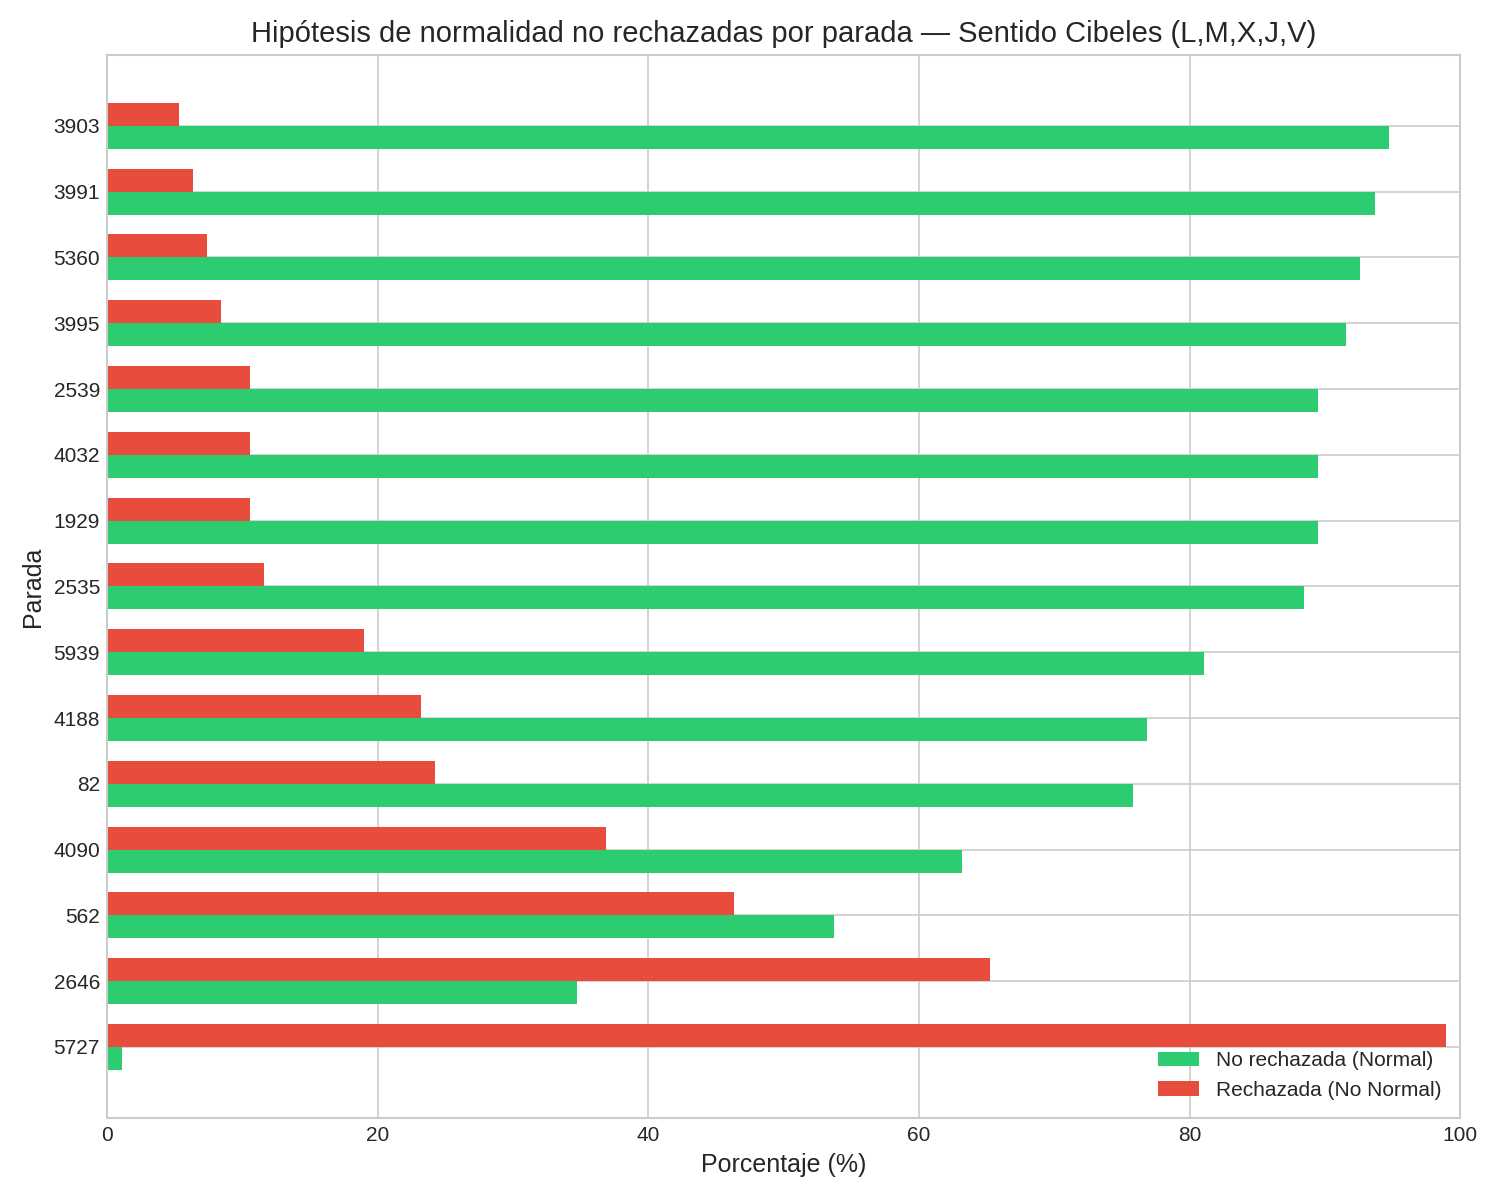
\includegraphics[width=\textwidth]{imagenes/to_A/normality_stop_individual.png}
\caption{Porcentaje de no rechazo de hipótesis de normalidad por parada en sentido Cibeles con datos desagregados.}
\par\vspace{4pt}{\footnotesize Fuente: elaboración propia.}\label{fig:normality_toA_deagregated}
\end{figure}

\begin{figure}[H]
 \centering
    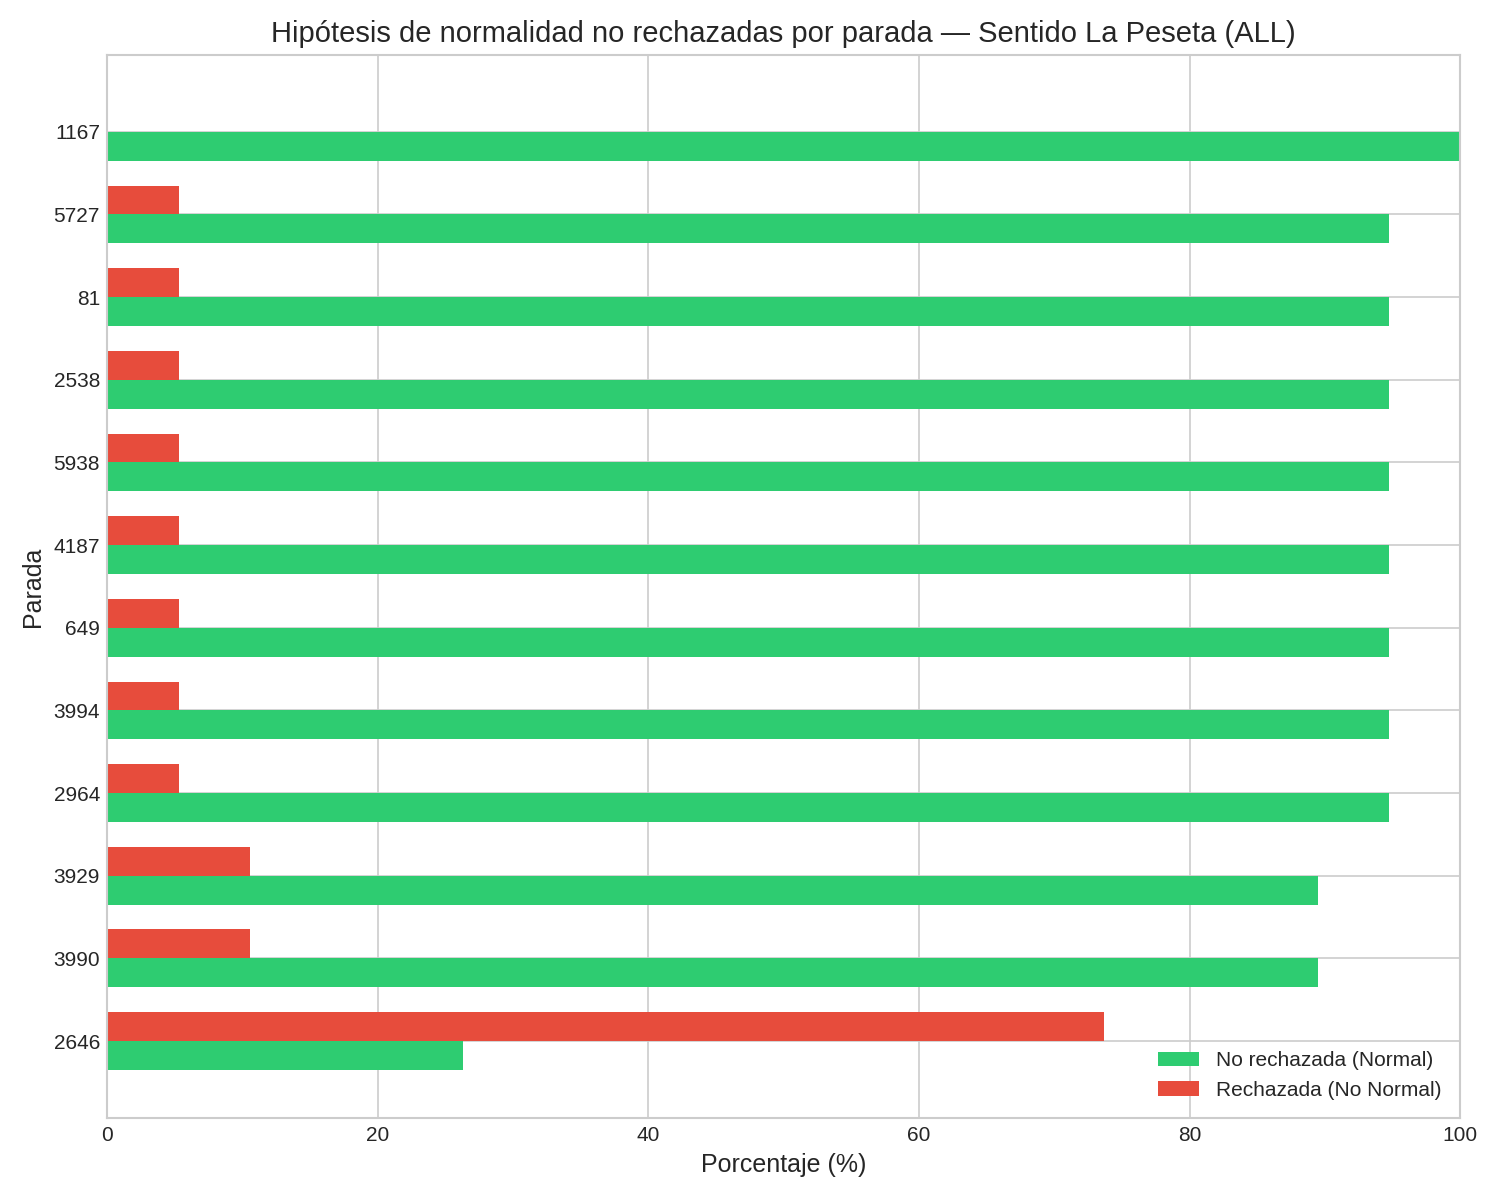
\includegraphics[width=\textwidth]{imagenes/to_B/normality_stop_ALL.png}
\caption{Porcentaje de no rechazo de hipótesis de normalidad por parada en sentido La Peseta con datos agregados.}
\par\vspace{4pt}{\footnotesize Fuente: elaboración propia.}\label{fig:normality_toB_all}
\end{figure}

\begin{figure}[H]
 \centering
    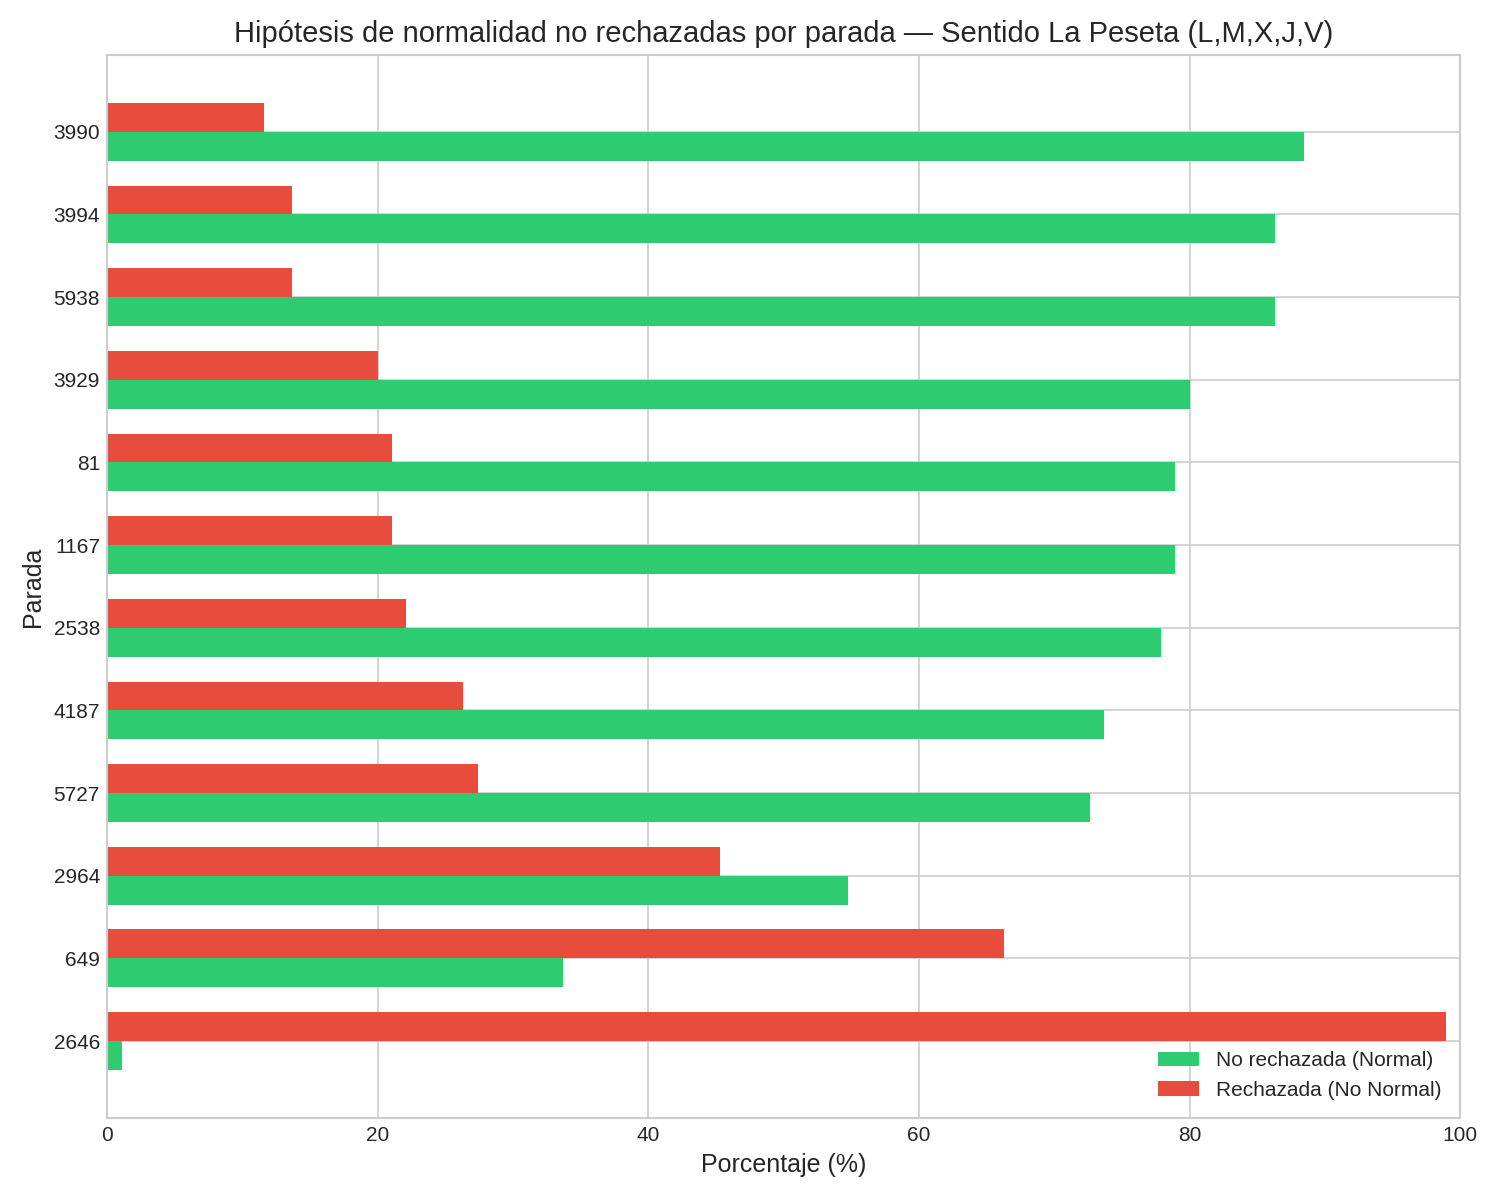
\includegraphics[width=\textwidth]{imagenes/to_B/normality_stop_individual.png}
\caption{Porcentaje de no rechazo de hipótesis de normalidad por parada en sentido La Peseta con datos desagregados.}
\par\vspace{4pt}{\footnotesize Fuente: elaboración propia.}\label{fig:normality_toB_deagregated}
\end{figure}